\documentclass[final,5p,times,authoryear]{elsarticle}

\usepackage{amsmath,amssymb}
\usepackage{booktabs}
\usepackage{graphicx}
\usepackage{url}
\usepackage{xcolor}
\usepackage{hyperref}
\usepackage{array}
\usepackage{placeins}
\usepackage{tikz}
\usetikzlibrary{positioning}

\hypersetup{hidelinks}

\emergencystretch=2em

\begin{document}

\begin{frontmatter}

\title{Contracting for Digital Product Passports: A Game-Theoretic Analysis of Supplier Data Sharing in Circular Supply Chains}

\author[inst1]{Patrick Boateng Sarpong\corref{cor1}}
\ead{psarpong@htu.edu.gh}
\author[inst2]{Daniel Commey}
\ead{ccommey@tamu.edu}
\author[inst3]{Benjamin Appiah}
\ead{bappiah@htu.edu.gh}
\author[inst4]{Godwin Banafo Akrong}
\ead{godwin.akrong@mail.mcgill.ca}

\affiliation[inst1]{organization={Department of Logistics and Supply Chain Management, Ho Technical University},
  city={Ho}, country={Ghana}}
\affiliation[inst2]{organization={Hung Family College of Engineering, California State University, Long Beach},
  city={Long Beach}, state={CA}, country={USA}}
\affiliation[inst3]{organization={Department of Computer Science, Ho Technical University},
  city={Ho}, country={Ghana}}
\affiliation[inst4]{organization={School of Information Studies, McGill University},
  city={Montreal}, country={Canada}}

\cortext[cor1]{Corresponding author.}

\begin{abstract}
Digital Product Passports (DPPs) are intended to make product, material, carbon, repairability, provenance, and end-of-life data available across circular supply chains. Their effectiveness, however, depends on suppliers that may face high data-collection costs, limited digital capability, audit exposure, and risks to commercially sensitive information. This paper models DPP disclosure as a sequential buyer--supplier contracting game. The buyer chooses a contract specifying audit probability, penalties, disclosure incentives, supplier support, and confidentiality protection; the supplier then chooses high-quality disclosure, low-quality disclosure, or non-disclosure. The model distinguishes mandatory DPP fields from more sensitive circularity fields that create greater downstream value but also higher disclosure risk. The analytical results show that audit and penalty clauses deter low-quality disclosure only when expected punishment exceeds the supplier's savings from partial disclosure, after accounting for incentives and reputational benefits. Supplier support and confidentiality protection can make high-quality disclosure more attractive, but they also impose costs on the buyer. Numerical simulations identify the contract regions in which basic compliance, incentive-only, audit/penalty, and hybrid contracts are buyer-preferred. Under the baseline parameterization, hybrid contracts perform best when supplier capability is low and buyer circularity value is high. Robustness checks show, however, that simpler contracts can dominate when governance costs are high, support is ineffective, or supplier capability is already strong. The paper contributes to circular supply-chain governance by showing that DPP data quality depends on contractual incentives and safeguards, not only on technical interoperability.
\end{abstract}

\begin{highlights}
\item DPP data sharing is modeled as a sequential buyer-supplier contracting game.
\item Supplier capability and confidentiality protections shape disclosure incentives.
\item Penalties deter partial disclosure only when expected punishment exceeds cost savings.
\item Hybrid contracts make high-quality disclosure more likely only when buyer value covers governance costs.
\item The model shows how specific DPP clauses affect suppliers' disclosure choices.
\end{highlights}

\begin{keyword}
Digital Product Passport \sep circular supply chains \sep supplier data sharing \sep contract theory \sep game theory \sep circular economy governance
\end{keyword}

\end{frontmatter}

\section{Introduction}

Digital Product Passports are emerging as a central tool for circular economy policy and industrial data governance. Under the European Union's Ecodesign for Sustainable Products Regulation, the DPP is intended to store product information that supports sustainability, circularity, and legal compliance \citep{eu2024espr}. For buyers and focal manufacturers, these data can support circular design, reuse, repair, remanufacturing, recycling, ESG reporting, and supply-chain risk management. For suppliers, the same requirements may create substantial costs and risks. A supplier may need to collect, structure, validate, and periodically update product-level information that has historically been fragmented across engineering systems, procurement records, quality documents, environmental calculations, and enterprise resource planning systems. Disclosure may also reveal commercially sensitive information about materials, processes, supplier networks, or cost structures.

The result is a strategic data-sharing problem. Buyers need trustworthy and verifiable DPP data, while suppliers may prefer partial disclosure, delayed disclosure, or non-disclosure when the private cost and risk of transparency are high. The practical question is therefore not only how to design a DPP data model, but how to make credible disclosure worthwhile for suppliers with different capabilities, risks, and outside options.

The analysis addresses two questions. First, when does a supplier prefer high-quality DPP disclosure over partial disclosure or non-disclosure? Second, when is it worthwhile for the buyer to use a hybrid contract that combines verification, incentives, confidentiality protection, and supplier support rather than relying on basic compliance, incentives alone, or audit-and-penalty clauses?

While prior work has established the value of DPP data for circular decision-making, less is known about the contractual conditions under which suppliers will provide complete, accurate, and verifiable data. A DPP mandate may still produce poor data if suppliers disclose only the minimum required fields, fear disclosure of sensitive information, or face only weak verification.

The paper contributes in three ways. First, it develops a DPP-specific contracting model in which data quality depends on supplier capability, disclosure cost, audit exposure, and commercial sensitivity. Second, it identifies two conditions that must hold for credible disclosure: low-quality disclosure must be unattractive, and high-quality disclosure must beat the supplier's outside option. Enforcement primarily addresses the first condition, while supplier support and confidentiality protection primarily address the second; incentives can contribute to both but do not substitute for verification when low-quality disclosure remains privately attractive. Third, the paper connects these analytical results to DPP contract design by showing how disclosure duties, audit rights, penalties, incentives, confidentiality protections, and capability-building provisions affect suppliers' disclosure choices.

\section{Literature Review}

\begin{table*}[t]
\centering
\begingroup
\setlength{\tabcolsep}{3pt}
\small
\caption{Literature summary and link to the analytical model.}
\label{tab:literature_summary}
\begin{tabular}{@{}p{0.21\linewidth}p{0.22\linewidth}p{0.30\linewidth}p{0.19\linewidth}@{}}
\toprule
Literature stream & Representative sources & Main insight & Use in model \\
\midrule
DPP data needs and ecosystem design & \citet{jensen2023digital}; \citet{king2023proposed}; \citet{lopes2024digital} & DPPs require interoperable product, material, environmental, and life-cycle data across supply-chain and reverse-logistics actors. & Motivates the buyer value term $R$ and the distinction between complete and partial disclosure. \\
DPP data governance & \citet{ducuing2023data}; \citet{eu2024espr} & DPP implementation depends on access rights, trust, data quality, legal compliance, and protection of sensitive information. & Motivates audit probability $p$, confidentiality protection, and supplier risk $r$. \\
Circular supply-chain governance & \citet{deangelis2018circular}; \citet{govindan2015reverse} & Circularity requires coordination across forward and reverse flows and depends on information for reuse, repair, remanufacturing, and recycling. & Links DPP data quality to circularity losses $L$ and residual value $\beta R$. \\
Contract theory and relational governance & \citet{cachon2003supply}; \citet{cachon2005supply}; \citet{poppo2002do}; \citet{malhotra2011trust} & Contracts can coordinate supply chains, allocate duties, and complement relational mechanisms when uncertainty and opportunism are present. & Supports comparison of incentive-only, enforcement-only, and hybrid governance. \\
Transaction cost economics and capability constraints & \citet{williamson2008outsourcing}; \citet{uruena2026digital} & Uncertainty, monitoring costs, asset specificity, and uneven digital capabilities shape governance choices. & Motivates capability $q$, support $S$, and monitoring cost $v$. \\
Sustainable supply-chain contracts and circularity & \citet{kolagar2026material}; \citet{doijjclepro201803046}; \citet{doijjclepro2022135135}; \citet{doijjclepro2021128629} & Prior work has used DPP readiness, game theory, coordination contracts, and empirical circular-supply-chain studies to examine sustainable supply-chain governance. & This paper extends that stream from DPP readiness, greening, and circular coordination to verifiable DPP data disclosure. \\
\bottomrule
\end{tabular}
\endgroup
\end{table*}

\subsection{DPPs and circular supply chains}

The DPP literature emphasizes that circular decisions require reliable product life-cycle information. \citet{jensen2023digital} identify data needs across product identification, materials, maintenance, environmental information, supply-chain and reverse-logistics information, and compliance. Their empirical evidence also shows that data availability and sensitivity vary across actors. \citet{king2023proposed} frame the DPP as a socio-technical ecosystem requiring interoperability across product life cycles, organizations, supply chains, and value chains. \citet{lopes2024digital} show that DPP research is still fragmented and that adoption challenges include data structure, technology choices, and supply-chain roles. These studies support the model's distinction between complete, decision-useful DPP data and partial disclosure that provides only residual value.

DPP disclosure differs from conventional supplier information sharing in several important ways. DPP data are product-level and machine-readable; they must often be linked to persistent identifiers, updated over the product life cycle, and made accessible to different actors under different access rights. Some fields are basic regulatory fields, such as product identification or mandatory compliance information. Other fields are strategic circularity fields, such as detailed material composition, repairability, process data, or recovery information. These fields are valuable for downstream circular decisions, but they may also reveal commercially sensitive information about materials, processes, or supplier relationships. The model therefore treats low-quality disclosure as a reduced-form representation of basic or weakly verifiable disclosure, while high-quality disclosure represents complete and verifiable DPP data that include strategic circularity fields.

\subsection{Supplier data sharing and information asymmetry}

DPPs require upstream suppliers to share information that downstream buyers cannot fully observe without verification. This produces information asymmetry and creates scope for opportunistic disclosure. A supplier may provide incomplete fields, unverifiable claims, stale records, or aggregated information that satisfies formal reporting requests while failing to support circular decisions. \citet{ducuing2023data} argue that DPPs raise data-governance challenges around access, trust, data quality, and the preservation of legally protected interests. These concerns motivate the model's audit probability, expected penalty, and confidentiality-adjusted commercial risk.

This setting also connects to inspection, audit, and information-sharing games. Prior game-theoretic work shows that verification changes strategic behavior only when monitoring probability and sanctions are strong enough to alter expected payoffs \citep{doi162583122023226544,doi002075432019168113}. Supply-chain information-sharing models similarly emphasize that data exchange is shaped by incentives, power, and the distribution of benefits \citep{doi002075432021192517,doijournalpone0298355}. The DPP case differs because the disclosed object is not a forecast or order signal but a verifiable product-level record with legal, circularity, and confidentiality consequences.

\subsection{Circular-economy contracting}

Circular supply chains require coordination across forward and reverse flows \citep{deangelis2018circular,govindan2015reverse}. Contract clauses can allocate responsibilities for disclosure, verification, repairability data, material composition, end-of-life obligations, and data updates. Recent work on circular-economy clauses highlights that contracting for circularity can shape market and financial outcomes \citep{castrolopez2026contracting}. In the DPP setting, clauses do not merely allocate legal responsibilities. They change the supplier's payoff from transparency, the buyer's ability to verify information, and the cost of building supplier data capability.

\begin{table*}[t]
\centering
\begingroup
\setlength{\tabcolsep}{3pt}
\tiny
\caption{DPP contract clause taxonomy.}
\label{tab:contract_clause_taxonomy}
\begin{tabular}{@{}p{0.20\textwidth}p{0.22\textwidth}p{0.12\textwidth}p{0.34\textwidth}@{}}
\toprule
Clause category & Contract function & Model link & Governance rationale \\
\midrule
Data disclosure requirements & Define mandatory DPP data fields & Disclosure duty & Creates a clear baseline duty to disclose. \\
Data quality and completeness requirements & Set accuracy and completeness thresholds & $C_H; C_L$ & Distinguishes high-quality disclosure from low-quality disclosure. \\
Material composition disclosure & Require composition transparency & $r$ & Addresses circular design and recycling information needs while raising IP sensitivity. \\
Carbon/environmental footprint disclosure & Require environmental metrics & $C_H$ & Supports ESG reporting and compliance but increases collection cost. \\
Repairability, reusability, and recyclability information & Support circular use decisions & $R$ & Converts DPP data into circular value for the buyer. \\
Data update frequency & Specify update timing & $C_H$ & Prevents stale disclosure and preserves compliance value. \\
Verification and audit rights & Permit buyer or third-party verification & $p; v$ & Creates detection probability for low-quality disclosure. \\
Third-party certification & Use independent assurance & $p; v; g$ & Increases credibility and reputational benefit of verified disclosure. \\
Penalties for false or incomplete data & Assign consequences for bad data & $F$ & Raises expected cost of low-quality disclosure. \\
Incentives for high-quality disclosure & Reward verified disclosure & $B$ & Increases supplier payoff from high-quality disclosure. \\
Data ownership and access rights & Allocate rights and permissions & $r$ & Reduces hold-up and misuse concerns. \\
Confidentiality and IP protection & Protect sensitive information & $r$ & Reduces commercial/IP risk from disclosure. \\
Cybersecurity and data protection & Secure DPP systems & $C_H; R$ & Maintains trustworthiness and operational resilience. \\
Supplier support and capability-building & Improve supplier readiness & $S; \alpha; q$ & Reduces high-quality disclosure cost especially for SMEs. \\
Extended producer responsibility and end-of-life obligations & Connect DPP data to circular duties & $R; L$ & Links DPP disclosure to reverse supply-chain performance. \\
Termination or preferred-supplier clauses & Set participation consequences & $O; B$ & Shapes the supplier participation constraint and outside option. \\
\bottomrule
\end{tabular}
\endgroup
\end{table*}

\subsection{Transaction cost economics and contract theory}

Transaction cost economics predicts that governance choices respond to uncertainty, monitoring costs, opportunism, and relationship specific investments \citep{williamson2008outsourcing}. DPP disclosure has all four features. Buyers face uncertainty about the accuracy and completeness of supplier data. Monitoring is costly. Suppliers may behave opportunistically when disclosure is expensive or commercially risky. Investments in data infrastructure and capability are partly relationship specific because they must match buyer schemas, regulatory product categories, and verification requirements.

Contract theory and supply-chain coordination research show that incentives can align decentralized decisions but may be limited when performance is hard to verify \citep{cachon2003supply,cachon2005supply}. Formal contracts can also complement relational governance rather than substitute for it \citep{poppo2002do,malhotra2011trust}. This is important for DPPs because the buyer often needs both formal audit rights and cooperative support mechanisms.

Supplier development research addresses the other side of the problem: whether suppliers have the capability and incentives to participate in the first place. Capability-building, collaboration, and relationship commitment can improve circular-economy outcomes, but they also consume buyer resources and may be targeted only to strategically important suppliers \citep{doibse3549,doi97813152330004}. In DPP contracting, support is therefore not a free add-on. It is an instrument that can lower supplier disclosure cost while creating a buyer-side investment cost.

The game-theory contribution also differs from standard sustainable supply-chain games. Greening, emission-reduction, CSR, and quality-inspection games typically model an effort choice whose output is valuable to the buyer or market. DPP disclosure is related but distinct: the supplier's action is the production of verifiable information about product attributes, and the buyer's problem is not only to induce effort but also to make sensitive, multi-field data credible, auditable, and usable for circular decisions. The model therefore combines incentive, inspection, confidentiality, and supplier-development instruments in one contract vector rather than studying a single greening or inspection lever.

\subsection{Dynamic capabilities and SME inclusion}

Supplier data capability is a central feature of the model. Dynamic capabilities matter because suppliers must sense data requirements, integrate internal systems, reconfigure data routines, and update disclosure over time. Firm size can shape digital circular-economy capability \citep{uruena2026digital}. This means uniform enforcement may be regressive: suppliers with low readiness face higher effective disclosure costs and may respond by withholding data or exiting the relationship.

\subsection{Positioning within circular-economy and sustainable supply-chain research}

This paper builds on research on circularity, sustainable supply-chain contracts, and digital circular-economy capabilities. \citet{king2023proposed} establish DPPs as socio-technical ecosystems and identify the need for incentives that encourage producers to share data. More recent DPP-specific work by \citet{kolagar2026material} shows that DPP readiness contributes to circular-economy performance only when it is embedded in wider configurations of business model innovation, social controls, and cooperation between organizations. \citet{uruena2026digital} show that digital-enabled dynamic capabilities support circular-economy implementation and that firm size conditions this relationship. In the sustainable supply-chain contract literature, \citet{doijjclepro201803046} use a two-stage game to compare contract types for greening and corporate social responsibility, while \citet{doijjclepro2022135135} connect coordination contracts to circular-economy and eco-innovation challenges. \citet{doijjclepro2021128629} further show that circular supply-chain implementation depends on drivers and capabilities that vary across firms. This paper extends that work by focusing not on greening effort, circular-economy adoption, DPP readiness, or ecosystem architecture, but on suppliers' strategic disclosure of verifiable DPP data. Its contribution is therefore not another general model of sustainable supply-chain coordination, but a DPP-specific account of how audit rights, penalties, incentives, confidentiality protections, and capability-building support shape data-quality equilibria.

\section{Model Development}

Consider a buyer that requires DPP data from a supplier to meet compliance obligations and support circular supply-chain decisions. The game has two stages. In Stage 1, the buyer chooses a contract vector $G_j=(p_j,F_j,B_j,B_{Lj},S_j,\phi_j)$ from a finite feasible set containing basic compliance, incentive-only, audit/penalty, and hybrid support contracts. In Stage 2, the supplier observes the selected vector and chooses high-quality disclosure $H$, low-quality disclosure $LQ$, or non-disclosure $N$.

Four assumptions structure the model. First, DPP data quality is only imperfectly contractible. Contracts can specify disclosure duties, audit rights, penalties, incentives, and support, but the buyer observes true data quality only through verification. Second, suppliers differ in their ability to produce complete, structured, and verifiable DPP data. Third, disclosure may expose commercially sensitive information, especially when it involves detailed material, process, provenance, or supplier-network data. Fourth, the buyer benefits from high-quality data because it supports compliance and circular decisions, while poor or missing data can lead to non-compliance, design errors, or failed recovery decisions.

To capture what is distinctive about DPPs, buyer value is separated into mandatory-field value $R_M$ and strategic circularity value $R_C$. Mandatory fields include product identity and compliance information; strategic fields include detailed material composition, repairability, process, recovery, or provenance information. High-quality disclosure yields $R=R_M+R_C$. Low-quality disclosure yields only residual value $\beta R$, with $\beta R$ corresponding to $R_M$ when low-quality disclosure is interpreted as mandatory-field-only compliance. Commercial sensitivity can be decomposed in the same way:
\begin{equation}
r_H=r_M+r_C(1-\phi),\qquad r_L=r_M+\rho r_C(1-\phi),\quad 0\leq\rho<1.
\end{equation}
The numerical model uses the normalized reduced form $r_M=0$ and denotes the strategic-field sensitivity $r_C$ by $r$. This keeps the simulation parsimonious while preserving the DPP distinction between basic compliance value and additional circularity value from strategic fields.

The buyer's contract instruments are bounded:
\begin{equation}
0\leq p\leq 1,\quad 0\leq F\leq \bar{F},\quad 0\leq S\leq \bar{S},\quad 0\leq \phi\leq 1.
\end{equation}
The bounds represent audit feasibility, legal and relational limits on penalties, finite supplier-development budgets, and feasible confidentiality/access-control protections. Table~\ref{tab:contract_vectors} reports the contract vectors used in the numerical model. These vectors should be interpreted as stylized contract packages, not as empirically calibrated contracts. Basic compliance contains small audit, penalty, and benefit terms to represent baseline regulatory clauses. Incentive-only raises the high-quality disclosure benefit while keeping verification and support low. Audit/penalty raises the expected enforcement term $pF$ while keeping support and confidentiality low. Hybrid support combines moderate enforcement with incentives, capability support, and confidentiality protection. Because supplier support is the only instrument that the buyer must actively resource, the support unit cost is treated as contract-specific: it is zero for the contracts that set $S_j=0$ (basic compliance, incentive-only, audit/penalty) and positive for the hybrid package ($k_H=0.8$), so that the hybrid contract internalizes the cost of the support it provides. The governance-cost sensitivity analysis later varies $k$ and the confidentiality cost coefficient $m$ jointly. The robustness checks perturb these packages to test whether the hybrid result is driven by the vector definitions.

\begin{table*}[t]
\centering
\begingroup
\setlength{\tabcolsep}{3pt}
\small
\caption{Discrete contract vectors used in the analytical and numerical model.}
\label{tab:contract_vectors}
\begin{tabular}{@{}p{0.28\linewidth}p{0.10\linewidth}p{0.10\linewidth}p{0.10\linewidth}p{0.10\linewidth}p{0.10\linewidth}p{0.10\linewidth}@{}}
\toprule
Contract & $p$ & $F$ & $B$ & $B_L$ & $S$ & $\phi$ \\
\midrule
Basic compliance & 0.05 & 1.00 & 0.25 & 0.10 & 0.00 & 0.10 \\
Incentive-only & 0.08 & 1.50 & 2.40 & 0.40 & 0.00 & 0.20 \\
Audit/penalty & 0.45 & 7.00 & 0.35 & 0.05 & 0.00 & 0.15 \\
Hybrid & 0.32 & 5.00 & 1.80 & 0.20 & 1.60 & 0.55 \\
\bottomrule
\end{tabular}
\endgroup
\end{table*}

Supplier capability is $q$, baseline high-quality data cost is $c$, and support effectiveness is $\alpha$. The main specification uses a bounded hyperbolic disclosure-cost function:
\begin{equation}
C_H=\max\left\{\frac{c}{q+\alpha S},\underline{C}\right\}.
\end{equation}
This specification allows capability and buyer support to reduce disclosure costs at a diminishing rate, while the floor $\underline{C}$ prevents disclosure from becoming costless. Robustness checks also use an affine form $C_H=\max\{c-\gamma q-\alpha S,\underline{C}\}$.
Low-quality disclosure is cheaper:
\begin{equation}
C_L=\lambda C_H, \quad 0<\lambda<1.
\end{equation}
Commercial risk terms $r_H$ and $r_L$ follow the field decomposition above. Low-quality disclosure reveals less strategic information, so its strategic-field risk exposure is lower than under high-quality disclosure.

The supplier receives gross relationship value $V$ from remaining with the buyer and outside-option payoff $O$ from non-disclosure. Supplier payoffs are:
\begin{align}
\pi_S(H)&=V+B+g-C_H-r_H,\\
\pi_S(LQ)&=V+B_L-C_L-pF-r_L,\\
\pi_S(N)&=O.
\end{align}
Here $g$ is the reputational benefit of verified disclosure.

The buyer receives value $R$ from high-quality DPP data. In DPP terms, $R$ combines the value of mandatory regulatory fields and strategic circularity fields. Low-quality data provides only residual value $\beta R$ and creates loss $L$ from poor decisions, circularity failure, or non-compliance. Audit cost is convex, $A(p)=vp^2$, reflecting the increasing marginal cost of more intensive verification. Support costs are $kS$, confidentiality and access-control costs are $M(\phi)=m\phi^2$, and any recoverable penalty share is $\eta pF$. Buyer payoffs are:
\begin{align}
\pi_B(H)&=R-B-vp^2-kS-m\phi^2,\\
\pi_B(LQ)&=\beta R-L-vp^2-B_L-kS-m\phi^2+\eta pF,\\
\pi_B(N)&=-L.
\end{align}
Verification, support, and confidentiality costs are incurred only conditional on an ongoing disclosure relationship: when the supplier exits, there is no record to audit, no support to deliver, and no protected data to safeguard, so the buyer bears only the loss $L$ from missing data. This keeps the buyer's outside-path payoff independent of the contract instruments and isolates the trade-off between inducing disclosure and paying for governance.

\begin{table*}[t]
\centering
\begingroup
\setlength{\tabcolsep}{3pt}
\small
\caption{Model parameters and default values.}
\label{tab:model_parameters}
\begin{tabular}{@{}p{0.16\linewidth}p{0.14\linewidth}p{0.62\linewidth}@{}}
\toprule
Parameter & Default & Interpretation \\
\midrule
$c$ & 5.0 & Supplier baseline cost of collecting, structuring, and validating high-quality DPP data. \\
Cost specification & hyperbolic & Disclosure cost form used in the simulation: hyperbolic main specification or affine robustness check. \\
$\underline{C}$ & 0.25 & Lower bound on high-quality disclosure cost. \\
$\gamma$ & 2.0 & Capability cost-reduction coefficient in the affine robustness specification. \\
$q$ & 0.6 & Supplier data capability/readiness level. \\
$r$ & 1.5 & Supplier commercial or IP risk from disclosure. \\
$p$ & 0.05 & Probability of buyer audit or verification. \\
$F$ & 1.0 & Penalty if low-quality disclosure is detected. \\
$\bar{F}$ & 10.0 & Maximum feasible penalty allowed by legal, relational, or enforceability constraints. \\
$B$ & 0.25 & Buyer premium or preferred-supplier benefit for high-quality disclosure. \\
$S$ & 0.0 & Buyer support or subsidy for supplier capability-building. \\
$\bar{S}$ & 3.0 & Maximum feasible buyer support level. \\
$R$ & 12.0 & Buyer value from high-quality DPP data. \\
$L$ & 5.0 & Buyer loss from poor data, circularity failure, or non-compliance. \\
$v$ & 1.0 & Buyer verification/audit cost coefficient. \\
$g$ & 0.8 & Supplier reputational gain from verified high-quality disclosure. \\
$k$ & 0.0 & Unit cost to the buyer of providing supplier support. \\
$m$ & 0.8 & Buyer cost coefficient for confidentiality and access-control protection. \\
$\alpha$ & 1.4 & Effectiveness of buyer support in reducing supplier disclosure cost. \\
$\lambda$ & 0.45 & Low-quality disclosure cost share relative to high-quality disclosure cost. \\
$\beta$ & 0.35 & Residual buyer value from low-quality or partial DPP data. \\
$\eta$ & 0.2 & Share of expected penalties that offsets buyer losses as recoverable damages. \\
$\rho$ & 0.35 & Commercial/IP risk share under low-quality disclosure. \\
$\phi$ & 0.1 & Strength of confidentiality and access-control protections. \\
$B_L$ & 0.1 & Supplier benefit from low-quality disclosure, such as continued transaction access. \\
$V$ & 7.0 & Supplier gross value from retaining the buyer relationship. \\
$O$ & 5.4 & Supplier payoff from non-disclosure and alternative opportunities. \\
\bottomrule
\end{tabular}
\endgroup
\end{table*}
\begin{table}[t]
\centering
\begingroup
\setlength{\tabcolsep}{3pt}
\small
\caption{Payoff matrix after the buyer selects a DPP governance contract.}
\label{tab:payoff_matrix}
\begin{tabular}{p{0.22\linewidth}p{0.34\linewidth}p{0.34\linewidth}}
\toprule
Supplier strategy & Supplier payoff & Buyer payoff \\
\midrule
High-quality disclosure & $V+B+g-C_H-r_H$ & $R-B-vp^2-kS-m\phi^2$ \\
Low-quality disclosure & $V+B_L-C_L-pF-r_L$ & $\beta R-L-vp^2-B_L-kS-m\phi^2+\eta pF$ \\
Non-disclosure & $O$ & $-L$ \\
\bottomrule
\end{tabular}
\endgroup
\end{table}

\section{Equilibrium Analysis}

The game is solved by backward induction, yielding a subgame-perfect equilibrium. For a given contract vector $G_j$, the supplier chooses the disclosure strategy with the highest payoff:
\begin{equation}
s_j^*\in\arg\max_{s\in\{H,LQ,N\}}\pi_S(s\mid G_j).
\end{equation}
Anticipating this response, the buyer chooses the contract with the highest induced payoff:
\begin{equation}
G^*\in\arg\max_{G_j\in\mathcal{G}}\pi_B(s_j^*\mid G_j),
\end{equation}
where $\mathcal{G}=\{G_{\mathrm{basic}},G_{\mathrm{inc}},G_{\mathrm{audit}},G_{\mathrm{hyb}}\}$ is the finite feasible set of contract packages.

Because both the supplier's action set $\{H,LQ,N\}$ and the buyer's feasible set $\mathcal{G}$ are finite, every subgame has a payoff-maximizing action and a subgame-perfect equilibrium in pure strategies exists. To make the equilibrium and the reported numerical statistics well defined when payoffs tie, we adopt the following tie-breaking convention: the supplier resolves indifference in favor of the higher-quality response, in the order $H\succ LQ\succ N$, and the buyer resolves indifference in favor of the lower-cost contract (and, if costs also tie, the less interventionist one). Under this convention the equilibrium contract and induced response are unique, which is the rule used to label the ``tie'' cases in the robustness tables. The buyer therefore chooses the contract package that maximizes its payoff after accounting for the supplier's best response. A hybrid contract $G_H$ is buyer-preferred to an alternative contract $G_a$ if and only if
\begin{equation}
\pi_B(s_H^*\mid G_H)\geq \pi_B(s_a^*\mid G_a).
\end{equation}
In particular, if the hybrid induces high-quality disclosure and an alternative induces non-disclosure, the hybrid is buyer-preferred when
\begin{equation}
R+L\geq B_H+v p_H^2+kS_H+m\phi_H^2.
\label{eq:hybrid_vs_none}
\end{equation}
Equation~\ref{eq:hybrid_vs_none} is the buyer-side counterpart to the supplier participation condition: inducing high-quality DPP data is worthwhile only when buyer circularity and compliance value exceed the full governance cost of the contract.

To simplify the buyer-side comparisons, define $A_j=vp_j^2$, $K_j=kS_j$, and $M_j=m\phi_j^2$ as the audit, support, and confidentiality costs under contract $G_j$. Table~\ref{tab:buyer_contract_comparisons} reports the most relevant pairwise buyer comparisons. The comparisons show when the hybrid contract is and is not optimal: when two contracts induce the same supplier response, the buyer prefers the lower-cost contract; when responses differ, the buyer trades off the added circularity value of high-quality DPP data against the extra governance cost required to induce it.

\begin{table*}[t]
\centering
\begingroup
\setlength{\tabcolsep}{3pt}
\small
\caption{Buyer-side contract comparison conditions.}
\label{tab:buyer_contract_comparisons}
\begin{tabular}{@{}p{0.22\linewidth}p{0.39\linewidth}p{0.31\linewidth}@{}}
\toprule
Comparison & Buyer-preference condition & Interpretation \\
\midrule
Hybrid $H$ vs. alternative $N$ & $R+L \geq B_H+A_H+K_H+M_H$ & Hybrid-induced high-quality disclosure is worthwhile only when DPP value plus avoided loss covers hybrid governance cost. \\
Hybrid $H$ vs. incentive $H$ & $B_H+A_H+K_H+M_H \leq B_I+A_I+K_I+M_I$ & If both contracts induce high-quality disclosure, the buyer prefers the lower-cost implementation package. \\
Hybrid $H$ vs. audit $LQ$ & $(1-\beta)R+L+A_A+B_{L,A}+K_A+M_A \geq B_H+A_H+K_H+M_H+\eta p_AF_A$ & Hybrid beats audit-induced partial disclosure when the added circularity value and avoided low-quality loss exceed the net extra cost. \\
Hybrid $H$ vs. basic $LQ$ & $(1-\beta)R+L+A_B+B_{L,B}+K_B+M_B \geq B_H+A_H+K_H+M_H+\eta p_BF_B$ & Hybrid beats basic compliance when complete data value offsets the extra incentive, audit, support, and confidentiality costs. \\
Audit $LQ$ vs. incentive $H$ & $(1-\beta)R+L+B_{L,A}+A_A+K_A+M_A-\eta p_AF_A \leq B_I+A_I+K_I+M_I$ & Audit-induced partial disclosure is buyer-preferred only when the cost of inducing high-quality disclosure is larger than the residual-value loss. \\
\bottomrule
\end{tabular}
\endgroup
\end{table*}

\begin{table*}[t]
\centering
\begingroup
\setlength{\tabcolsep}{3pt}
\small
\caption{Supplier equilibrium conditions in the DPP disclosure game.}
\label{tab:equilibrium_conditions}
\begin{tabular}{p{0.22\linewidth}p{0.34\linewidth}p{0.34\linewidth}}
\toprule
Equilibrium object & Condition & Interpretation \\
\midrule
High-quality disclosure & $pF+(B-B_L)+g \geq (1-\lambda)C_H+(r_H-r_L)$ and $V+B+g-C_H-r_H \geq O$ & Supplier chooses high-quality DPP data when the combined incentive, reputation, and expected enforcement advantage exceeds the cost saving and risk advantage of partial disclosure, and participation beats the outside option. \\
Low-quality disclosure & $pF+(B-B_L)+g < (1-\lambda)C_H+(r_H-r_L)$ and $V+B_L-C_L-pF-r_L \geq O$ & Partial disclosure is selected when shirking remains cheaper than complete disclosure after expected penalties, but staying in the buyer relationship still beats non-disclosure. \\
Non-disclosure & $O>V+B+g-C_H-r_H$ and $O>V+B_L-C_L-pF-r_L$ & The supplier exits or refuses DPP disclosure when both disclosure strategies fall below the outside option. \\
Audit deterrence threshold & $pF \geq (C_H-C_L)+(r_H-r_L)-(B-B_L)-g$ & Audit and penalty clauses deter low-quality disclosure only when expected punishment covers the supplier's savings from lower-quality data net of incentives and reputation. \\
Support threshold & $C_H(q,S)\leq V+B+g-r_H-O$ & Capability-building support makes high-quality disclosure feasible by lowering the effective disclosure cost enough to satisfy participation. \\
\bottomrule
\end{tabular}
\endgroup
\end{table*}

\textbf{Proposition 1 (Deterrence condition).} For any feasible contract vector, high-quality disclosure gives the supplier at least as high a payoff as low-quality disclosure, $\pi_S(H)\geq\pi_S(LQ)$, if and only if
\[
pF+(B-B_L)+g \geq (C_H-C_L)+(r_H-r_L).
\]

\textit{Proof.} See \ref{app:proofs}.

\textbf{Proposition 2 (Best response).} High-quality disclosure is the supplier's best response to a contract vector if and only if the deterrence condition in Proposition~1 holds and the participation constraint
\[
V+B+g-C_H-r_H\geq O
\]
is satisfied.

\textit{Proof.} See \ref{app:proofs}.

\textbf{Proposition 3.} Higher supplier capability $q$ and buyer support $S$ expand the region in which high-quality disclosure is chosen, provided they reduce $C_H$ without lowering the supplier's disclosure benefit.

\textit{Proof.} See \ref{app:proofs}.

\textbf{Proposition 4.} Incentive-only contracts can improve participation, but they do not ensure data quality when the expected enforcement term $pF$ is too small to offset the cost and risk advantage of partial disclosure.

\textit{Proof.} See \ref{app:proofs}.

\textbf{Proposition 5.} A hybrid contract that induces high-quality disclosure is buyer-preferred to non-disclosure if and only if Equation~\ref{eq:hybrid_vs_none} holds. It is buyer-preferred to any other contract $G_a$ if and only if $\pi_B(H\mid G_H)\geq \pi_B(s_a^*\mid G_a)$.

\textit{Proof.} See \ref{app:proofs}.

\textbf{Proposition 6.} High commercial or IP risk can prevent high-quality disclosure even when penalties are strong. Data-access restrictions and confidentiality protections can reduce that risk, but they are worthwhile for the buyer only when the resulting disclosure benefit exceeds their governance cost.

\textit{Proof.} See \ref{app:proofs}.

\section{Numerical Simulation}

The numerical analysis evaluates supplier best responses and buyer-optimal contract choices across parameter grids for the four contract packages. The baseline grid varies capability $q$, disclosure cost $c$, commercial risk $r$, buyer value $R$, and the supplier outside option $O$. Additional experiments vary audit probability and penalty, capability and support, disclosure cost and risk, buyer value and audit cost, support cost $k$, confidentiality cost $m$, support effectiveness $\alpha$, relationship value $V$, and the disclosure-cost specification.

\begin{figure*}[!htpb]
\centering
\resizebox{\textwidth}{!}{%
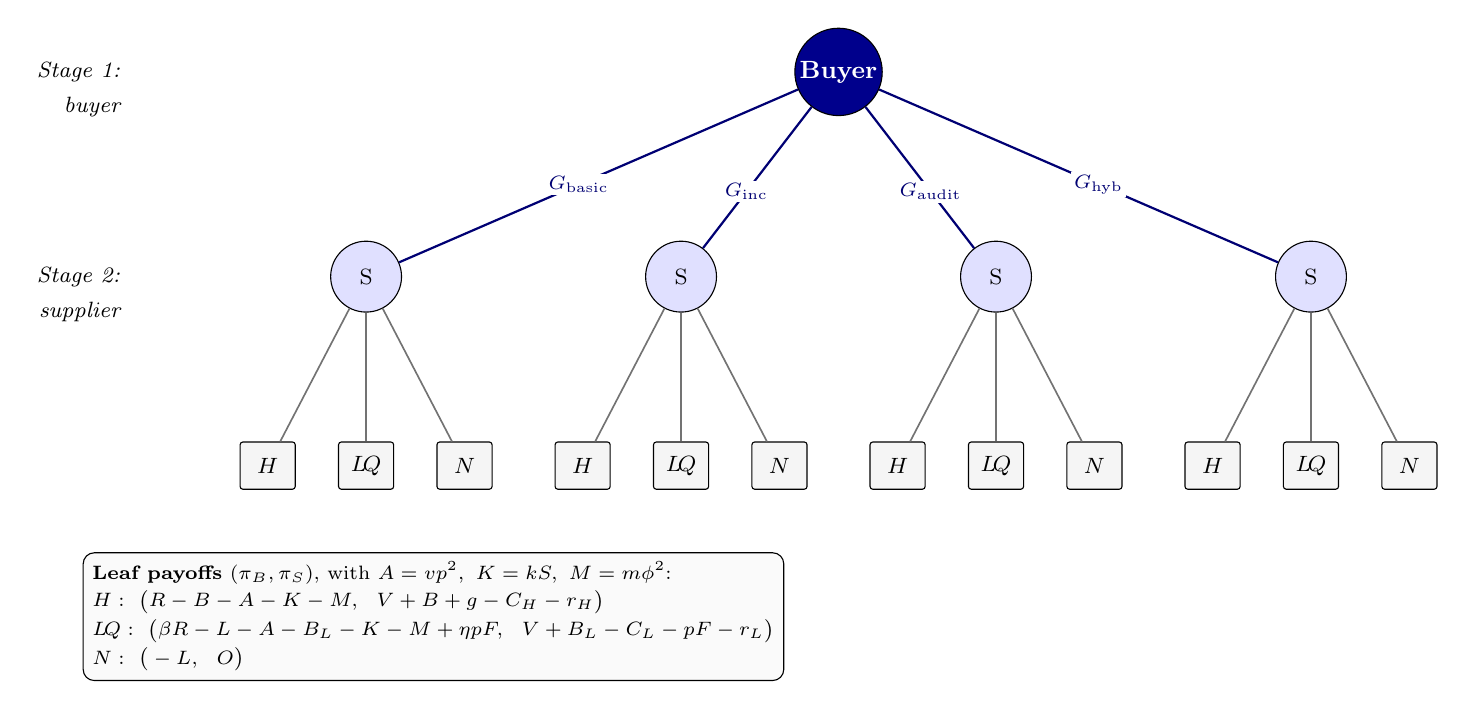
\begin{tikzpicture}[
    every node/.style={font=\small},
    buyer/.style={circle,draw,fill=blue!55!black,text=white,minimum size=10mm,inner sep=1pt,font=\small\bfseries},
    supp/.style={circle,draw,fill=blue!12,minimum size=9mm,inner sep=1pt,font=\footnotesize},
    leaf/.style={rectangle,draw,fill=black!4,rounded corners=1pt,minimum width=7mm,minimum height=6mm,font=\footnotesize},
    contractedge/.style={thick,blue!45!black},
    actionedge/.style={semithick,black!55},
    elabel/.style={font=\scriptsize,fill=white,inner sep=1pt},
]
\node[buyer] (B) at (8,0) {Buyer};
\node[supp] (S1) at (2,-2.6)  {S};
\node[supp] (S2) at (6,-2.6)  {S};
\node[supp] (S3) at (10,-2.6) {S};
\node[supp] (S4) at (14,-2.6) {S};
\draw[contractedge] (B) -- (S1) node[elabel,pos=0.55]{$G_{\mathrm{basic}}$};
\draw[contractedge] (B) -- (S2) node[elabel,pos=0.6]{$G_{\mathrm{inc}}$};
\draw[contractedge] (B) -- (S3) node[elabel,pos=0.6]{$G_{\mathrm{audit}}$};
\draw[contractedge] (B) -- (S4) node[elabel,pos=0.55]{$G_{\mathrm{hyb}}$};
\foreach \sx/\g in {2/1, 6/2, 10/3, 14/4}{
  \node[leaf] (H\g) at (\sx-1.25,-5.0) {$H$};
  \node[leaf] (L\g) at (\sx,-5.0)      {$L\!Q$};
  \node[leaf] (N\g) at (\sx+1.25,-5.0) {$N$};
}
\foreach \g in {1,2,3,4}{
  \draw[actionedge] (S\g) -- (H\g);
  \draw[actionedge] (S\g) -- (L\g);
  \draw[actionedge] (S\g) -- (N\g);
}
\node[anchor=east,font=\footnotesize\itshape] at (-1.0,0) {Stage 1:};
\node[anchor=east,font=\footnotesize\itshape] at (-1.0,-0.45) {buyer};
\node[anchor=east,font=\footnotesize\itshape] at (-1.0,-2.6) {Stage 2:};
\node[anchor=east,font=\footnotesize\itshape] at (-1.0,-3.05) {supplier};
\node[draw,rounded corners,align=left,font=\scriptsize,anchor=north west,fill=black!2] at (-1.6,-6.1)
  {\textbf{Leaf payoffs} $(\pi_B,\pi_S)$, with $A=vp^2,\ K=kS,\ M=m\phi^2$:\\[2pt]
   $H:\ \big(R-B-A-K-M,\ \ V+B+g-C_H-r_H\big)$\\[1pt]
   $L\!Q:\ \big(\beta R-L-A-B_L-K-M+\eta pF,\ \ V+B_L-C_L-pF-r_L\big)$\\[1pt]
   $N:\ \big(-L,\ \ O\big)$};
\end{tikzpicture}%
}
\caption{Extensive form of the sequential buyer--supplier DPP contracting game. In Stage~1 the buyer selects a contract vector $G_j\in\mathcal{G}$; in Stage~2 the supplier chooses high-quality disclosure ($H$), low-quality disclosure ($LQ$), or non-disclosure ($N$). Leaf payoffs are common across contracts and are listed in the key (see also Table~\ref{tab:payoff_matrix}).}
\label{fig:game_tree}
\end{figure*}

\begin{figure*}[!htpb]
\centering
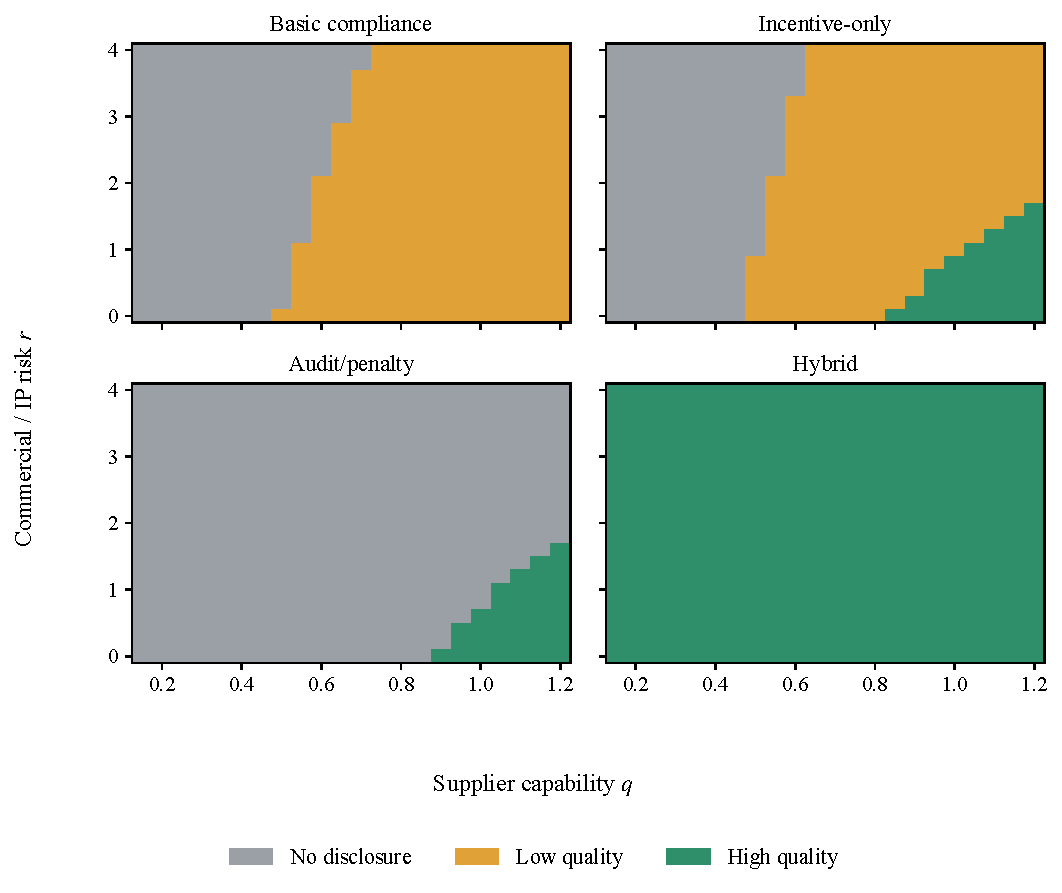
\includegraphics[width=\linewidth]{figures/fig_equilibrium_regions.pdf}
\caption{Equilibrium disclosure regions by contract type.}
\label{fig:equilibrium_regions}
\end{figure*}

Figure~\ref{fig:equilibrium_regions} shows how capability and commercial risk shape supplier disclosure under each contract package. Basic compliance leaves a large low-quality or non-disclosure region when supplier capability is low or commercial risk is high. Incentive-only contracting expands high-quality disclosure but does not fully eliminate low-quality disclosure. Audit/penalty contracting reduces partial disclosure where expected punishment is high enough, but it can also leave suppliers at the participation boundary. Hybrid support expands high-quality disclosure by lowering cost and risk rather than relying only on punishment.

\begin{figure*}[!htpb]
\centering
\begin{minipage}[t]{0.48\textwidth}
\centering
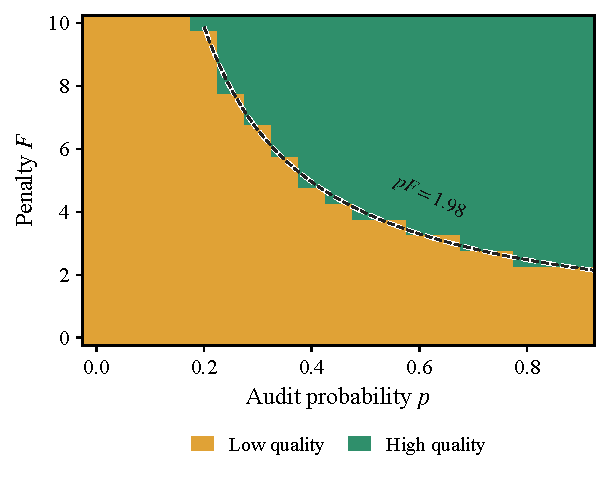
\includegraphics[width=\linewidth]{figures/fig_audit_penalty_heatmap.pdf}
\small (a) Audit probability and penalty.
\end{minipage}
\hfill
\begin{minipage}[t]{0.48\textwidth}
\centering
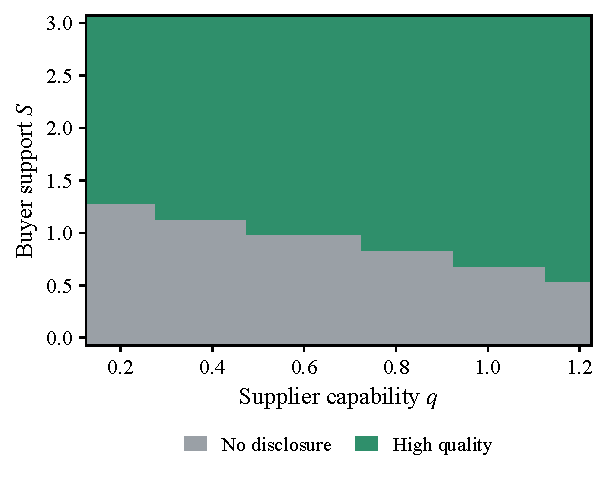
\includegraphics[width=\linewidth]{figures/fig_capability_support_heatmap.pdf}
\small (b) Supplier capability and buyer support.
\end{minipage}
\caption{Threshold heatmaps for audit deterrence and hybrid support.}
\label{fig:threshold_heatmaps}
\end{figure*}

The left panel of Figure~\ref{fig:threshold_heatmaps} illustrates the deterrence threshold of Proposition~1. The dashed curve is the analytical boundary $pF=(C_H-C_L)+(r_H-r_L)-(B-B_L)-g$, and it coincides with the simulated switch from low-quality to high-quality disclosure. Higher penalties have little effect when audit probability is very low, and high audit probability has limited effect if penalties are trivial: enforcement works through the expected penalty $pF$, not through either component in isolation.

The right panel of Figure~\ref{fig:threshold_heatmaps} shows why low-capability suppliers may require support before high-quality disclosure becomes privately attractive. As capability increases, the amount of support required to cross the participation boundary declines.

\begin{figure*}[!htpb]
\centering
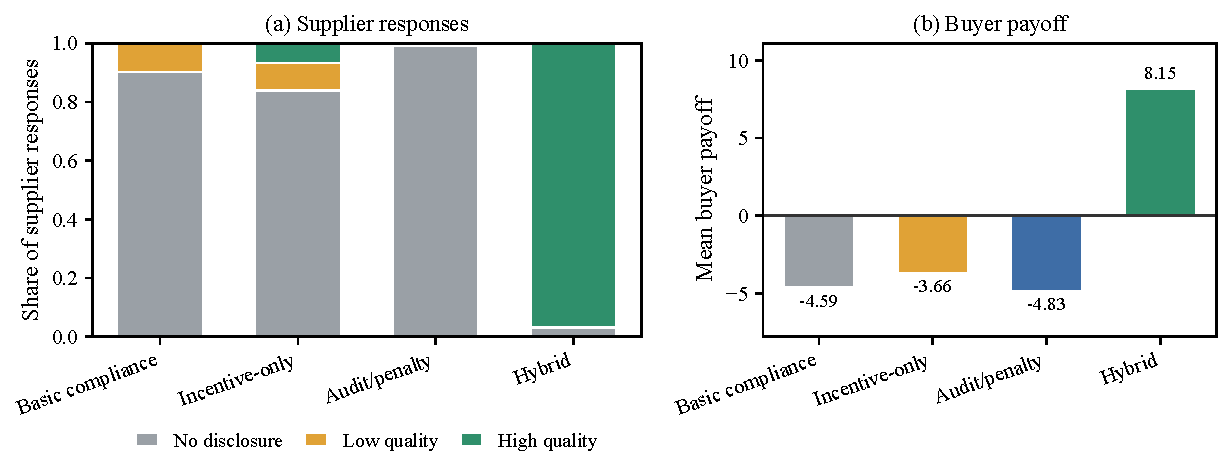
\includegraphics[width=\linewidth]{figures/fig_contract_comparison.pdf}
\caption{Contract comparison across the baseline grid.}
\label{fig:contract_comparison}
\end{figure*}

\begin{table*}[t]
\centering
\begingroup
\setlength{\tabcolsep}{3pt}
\small
\caption{Contract scenario comparison across the baseline parameter grid.}
\label{tab:contract_scenario_comparison}
\begin{tabular}{@{}p{0.21\linewidth}p{0.12\linewidth}p{0.12\linewidth}p{0.12\linewidth}p{0.17\linewidth}p{0.18\linewidth}@{}}
\toprule
Contract & High & Low & None & Buyer payoff & Supplier payoff \\
\midrule
Basic compliance & 0.0\% & 9.9\% & 90.1\% & -4.59 & 4.85 \\
Incentive-only & 6.8\% & 9.4\% & 83.9\% & -3.66 & 4.92 \\
Audit/penalty & 1.0\% & 0.0\% & 99.0\% & -4.83 & 4.80 \\
Hybrid & 96.9\% & 0.0\% & 3.1\% & 8.15 & 6.72 \\
\bottomrule
\end{tabular}
\endgroup
\end{table*}

Under the stated parameterization, hybrid contracts induce high-quality disclosure in most baseline cases because they act on both the deterrence and the participation margins. This advantage is specific to the baseline parameters; the robustness checks below identify the conditions under which it disappears.

\begin{figure*}[!htpb]
\centering
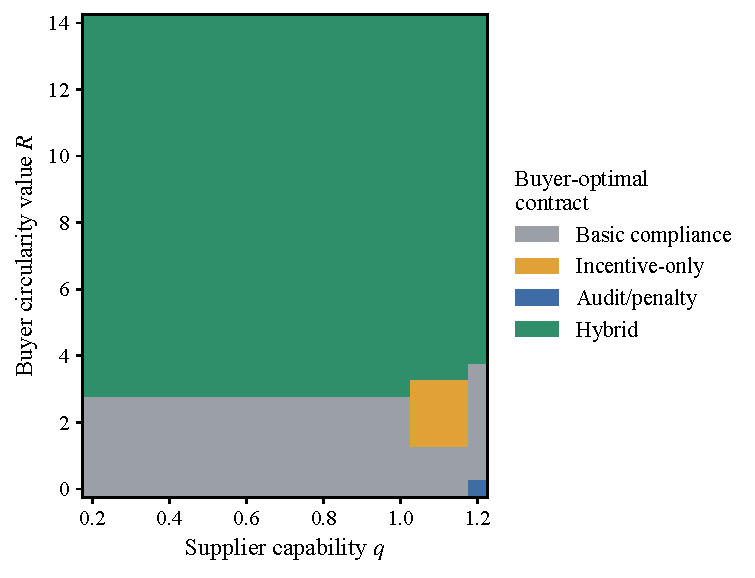
\includegraphics[width=\linewidth]{figures/fig_buyer_choice_region.pdf}
\caption{Buyer-optimal contract by supplier capability and buyer circularity value.}
\label{fig:buyer_choice_region}
\end{figure*}

Figure~\ref{fig:buyer_choice_region} maps the buyer's preferred contract after anticipating supplier best responses. Hybrid contracting is most attractive when the buyer's circularity value is high enough to cover incentive, support, audit, and confidentiality costs. When buyer value is low, basic compliance or less intensive contracts can be preferred because the additional governance expenditure is not justified.

\begin{figure*}[!htpb]
\centering
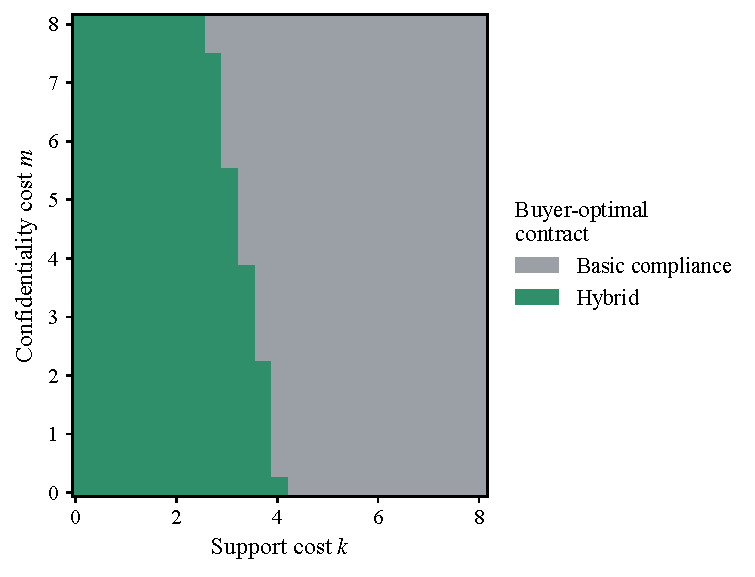
\includegraphics[width=\linewidth]{figures/fig_governance_cost_sensitivity.pdf}
\caption{Buyer-optimal contract under support-cost and confidentiality-cost sensitivity.}
\label{fig:governance_cost_sensitivity}
\end{figure*}

Figure~\ref{fig:governance_cost_sensitivity} shows when the cost of support and confidentiality protection outweighs the benefit of inducing high-quality disclosure. As support cost $k$ and confidentiality cost $m$ rise, the buyer increasingly prefers basic compliance over a full hybrid package, reflecting that confidentiality protection and supplier support are costly instruments rather than free additions.

\FloatBarrier

\begin{table*}[t]
\centering
\begingroup
\setlength{\tabcolsep}{3pt}
\small
\caption{Monte Carlo buyer-optimal contract robustness by disclosure-cost specification.}
\label{tab:monte_carlo_buyer_choice}
\begin{tabular}{@{}p{0.16\linewidth}p{0.12\linewidth}p{0.13\linewidth}p{0.12\linewidth}p{0.12\linewidth}p{0.19\linewidth}p{0.08\linewidth}@{}}
\toprule
Cost form & Basic & Incentive & Audit & Hybrid & Mean buyer payoff & $n$ \\
\midrule
Affine & 15.3\% & 10.7\% & 20.0\% & 54.0\% & 7.56 & 600 \\
Hyperbolic & 7.0\% & 1.7\% & 4.2\% & 87.2\% & 7.88 & 600 \\
\bottomrule
\end{tabular}
\endgroup
\end{table*}
\FloatBarrier

Table~\ref{tab:monte_carlo_buyer_choice} reports a Monte Carlo robustness check with random draws over supplier capability, disclosure cost, commercial risk, buyer value, loss from poor data, audit cost, support cost, confidentiality cost, relationship value, and outside option. Hybrid remains the most frequently buyer-optimal contract, but it does not dominate across the whole parameter space. Under the affine disclosure-cost specification, audit/penalty, basic compliance, and incentive-only contracts are buyer-optimal in non-trivial regions of the parameter space.

\begin{table*}[t]
\centering
\begingroup
\setlength{\tabcolsep}{3pt}
\small
\caption{Targeted robustness cases where the buyer need not prefer hybrid support.}
\label{tab:targeted_robustness}
\begin{tabular}{@{}p{0.17\linewidth}p{0.27\linewidth}p{0.16\linewidth}p{0.09\linewidth}p{0.09\linewidth}p{0.09\linewidth}@{}}
\toprule
Robustness case & Perturbation & Buyer-optimal contract & Response & Best payoff & Hybrid payoff \\
\midrule
Hybrid no support & Set hybrid support to zero for a low-capability supplier. & Basic compliance (tie) & None & -5.00 & -5.00 \\
High governance cost & Raise buyer costs for support and confidentiality protection. & Basic compliance (tie) & None & -3.50 & -10.61 \\
Low support effectiveness & Reduce alpha so support barely lowers disclosure cost. & Basic compliance (tie) & None & -4.50 & -4.50 \\
High relationship value & Increase relationship value so support is less necessary. & Audit/penalty & High & 8.43 & 5.58 \\
High capability & Raise capability so supplier support has low marginal value. & Audit/penalty & High & 8.43 & 5.58 \\
Incentives sufficient & Use moderate risk and high governance costs where incentives induce H. & Incentive-only & High & 7.93 & 1.23 \\
\bottomrule
\end{tabular}
\endgroup
\end{table*}
\FloatBarrier

Table~\ref{tab:targeted_robustness} reports targeted stress tests. Removing support from the hybrid package eliminates the mechanism that helps low-capability suppliers satisfy participation. High support or confidentiality costs make basic compliance preferable even when hybrid can induce high-quality disclosure. When support is ineffective, no contract can profitably induce disclosure under the tested low-capability setting. For high-capability suppliers or suppliers that already value the relationship, audit/penalty can be sufficient because the buyer does not need to pay for support. In a moderate-risk case with high governance costs, incentive-only contracting induces high-quality disclosure at lower buyer cost than hybrid support. Together these cases show that the baseline hybrid result is conditional on support effectiveness, capability, relationship value, and buyer governance cost.

\FloatBarrier

\clearpage

\section{Discussion}

The results indicate that DPP data quality depends on two distinct conditions. First, low-quality disclosure must be unattractive. Buyers can influence this deterrence margin through audit rights, penalties, and reputational consequences. Second, high-quality disclosure must be feasible and worthwhile for the supplier. Buyers can influence this participation margin through incentives, supplier support, and confidentiality protection.

This distinction explains why no single contractual instrument is sufficient in all settings. Enforcement-only contracts may discourage partial disclosure, but they can also push low-capability suppliers toward non-disclosure if complete data are too costly to produce. Incentive-only contracts can make participation more attractive, but they may reward disclosure without ensuring that the data are complete and verifiable. Hybrid contracts address both margins, but only when the value of high-quality DPP data justifies the combined cost of incentives, audits, support, and confidentiality safeguards.

The broader implication is that DPP implementation cannot be reduced to data standards or digital infrastructure. Even with a clear schema, suppliers may under-disclose when complete data are costly, commercially sensitive, or weakly verified. At the same time, buyers should not automatically choose the most elaborate contract. Effective DPP governance requires matching the contract to the supplier's capability, the sensitivity of the data, the buyer's circularity value, and the cost of verification and support.

\section{Managerial Implications}

\begin{table*}[t]
\centering
\begingroup
\setlength{\tabcolsep}{3pt}
\small
\caption{Managerial implications from the DPP contracting game.}
\label{tab:managerial_implications}
\begin{tabular}{@{}p{0.24\linewidth}p{0.34\linewidth}p{0.34\linewidth}@{}}
\toprule
Governance problem & Model implication & Managerial action \\
\midrule
Low supplier capability & Penalties can induce exit or non-disclosure when suppliers cannot cheaply generate complete data. & Pair DPP obligations with templates, onboarding, shared data infrastructure, and phased capability-building. \\
High commercial/IP sensitivity & Suppliers may resist complete disclosure even under strong audit rights. & Use access tiers, confidentiality protections, field-level permissions, and purpose limitation. \\
Weak verification & Incentives may buy participation without assuring data quality. & Tie premiums or preferred-supplier status to verifiable completeness and audit trails. \\
SME-heavy supplier base & Uniform enforcement shifts compliance burdens to least capable firms. & Segment suppliers by readiness and use hybrid support for strategically important SME suppliers. \\
High buyer circularity value & The value of trustworthy DPP data can justify support and verification costs. & Evaluate DPP contracting as circular supply-chain investment rather than administrative compliance. \\
\bottomrule
\end{tabular}
\endgroup
\end{table*}

For buyers, DPP contract design should begin with a diagnosis of the supplier's likely disclosure barrier. If the main problem is weak verification, incentives should be tied to audit trails, certification, or other evidence of data completeness. If the main problem is low supplier capability, penalties alone may be counterproductive; templates, onboarding, shared infrastructure, or phased implementation may be needed. If the main problem is commercial sensitivity, the contract should specify access tiers, purpose limitations, confidentiality obligations, and safeguards for sensitive fields.

The model also suggests that buyers should segment suppliers rather than impose a uniform DPP contract across the supply base. High-capability suppliers may require only verification and modest incentives. Low-capability but strategically important suppliers may justify support. Suppliers handling highly sensitive data may require stronger confidentiality protections before complete disclosure is feasible. In this sense, DPP contracting is not merely a compliance exercise; it is a supplier-governance decision.

\section{Policy Implications}

For policymakers, the model highlights a potential weakness in DPP mandates. Requiring more granular product and material data does not guarantee that suppliers can provide reliable, verifiable, and decision-useful information. Smaller or less digitally mature suppliers may face disproportionate compliance burdens, especially when required data are dispersed across engineering, procurement, quality, and environmental systems.

Policy support should therefore address the conditions under which credible disclosure is possible. Standardized templates, interoperable data infrastructures, assurance protocols, and guidance on confidential business information can reduce disclosure costs and risks. Without these complementary measures, DPP regulation may produce formal compliance while leaving buyers with incomplete or weakly verifiable data.

\section{Limitations and Future Research}

The model is parsimonious. It considers one buyer and one supplier, assumes complete information about key parameters, and restricts the buyer's choice to a finite set of contract packages. These assumptions make the main mechanism transparent, but they also limit the scope of the results.

Future research could relax these assumptions in several ways. A Bayesian model could examine how buyers contract when supplier capability, disclosure cost, or commercial risk is uncertain. A repeated-game setting could capture how disclosure quality affects trust, renewal, and relational rents over time. Multi-tier models could examine DPP data that must pass through several suppliers before reaching the buyer. Mechanism-design approaches could study how buyers screen suppliers by offering different combinations of audit intensity, support, incentives, and confidentiality protection. Empirical work could also test the contract-clause taxonomy and estimate plausible parameter ranges from DPP pilots or procurement data.

\section{Conclusion}

Digital Product Passports are often presented as tools for transparency and circularity. This paper shows that such transparency depends on the incentives and safeguards surrounding supplier disclosure. Suppliers provide high-quality DPP data only when verified disclosure offers sufficient benefits relative to data-collection costs, audit exposure, and commercial sensitivity.

The model identifies two conditions for credible disclosure. Low-quality disclosure must be deterred, and high-quality disclosure must be attractive relative to non-disclosure. Penalties can help with deterrence, but they do not solve weak supplier capability. Incentives can improve participation, but they do not by themselves guarantee verifiable data quality. Confidentiality protections and supplier support can expand the conditions under which complete disclosure is feasible, but they are worthwhile for the buyer only when the value of reliable DPP data exceeds the cost of governance.

Under the baseline parameterization, hybrid contracts are especially effective when supplier capability is low and buyer circularity value is high. Robustness checks show that simpler contracts may be preferred when governance costs are high, support is ineffective, or suppliers already have strong disclosure capability. The paper therefore contributes a contracting perspective on DPP governance: credible circularity data require not only technical standards, but also contractual mechanisms that align supplier incentives with buyer data needs.

\section*{Code and data availability}

The code is available at \href{https://github.com/dcommey/dpp-contracting-game}{https://github.com/dcommey/dpp-contracting-game}.

\section*{Declaration of competing interest}

The authors declare no known competing financial interests or personal relationships that could have appeared to influence the work reported in this paper.

\appendix
\section{Proofs of Analytical Results}
\label{app:proofs}

\textbf{Proof of Proposition 1.} Fix any feasible contract vector $G=(p,F,B,B_L,S,\phi)$ and the induced cost and risk terms. High-quality disclosure is at least as profitable as low-quality disclosure for the supplier if and only if $\pi_S(H)\geq \pi_S(LQ)$. Substituting the supplier payoff functions gives
\[
V+B+g-C_H-r_H \geq V+B_L-C_L-pF-r_L .
\]
Canceling the common relationship value $V$ and collecting incentive, reputation, and enforcement terms on the left yields
\[
pF+(B-B_L)+g \geq (C_H-C_L)+(r_H-r_L).
\]
This proves necessity because every algebraic step is reversible. It proves sufficiency because, if the final inequality holds, reversing the same steps gives $\pi_S(H)\geq\pi_S(LQ)$. Since $C_L=\lambda C_H$ with $0<\lambda<1$, the cost term can equivalently be written as $(1-\lambda)C_H$. The result therefore characterizes exactly the deterrence constraint separating high-quality disclosure from partial disclosure.

\textbf{Proof of Proposition 2.} The supplier's feasible strategy set is finite: $\{H,LQ,N\}$. Hence $H$ is a best response if and only if it yields at least as high a payoff as each alternative. Proposition 1 gives the necessary and sufficient condition for $\pi_S(H)\geq\pi_S(LQ)$. The condition for high-quality disclosure to be at least as profitable as non-disclosure is
\[
\pi_S(H)\geq\pi_S(N)
\iff
V+B+g-C_H-r_H\geq O .
\]
If both inequalities hold, then $\pi_S(H)$ is at least as large as the payoff from every feasible supplier action, so $H\in\arg\max_{s\in\{H,LQ,N\}}\pi_S(s\mid G)$. Conversely, if $H$ is a best response, it must yield at least as high a payoff as $LQ$ and $N$; otherwise either $LQ$ or $N$ would yield a strictly higher payoff. The two inequalities are therefore jointly necessary and sufficient. The first is the deterrence constraint and the second is the participation constraint.

\textbf{Proof of Proposition 3.} In the main specification,
\[
C_H(q,S)=\max\left\{\frac{c}{q+\alpha S},\underline{C}\right\}.
\]
For any region in which the floor does not bind,
\[
\frac{\partial C_H}{\partial q}=-\frac{c}{(q+\alpha S)^2}<0,\qquad
\frac{\partial C_H}{\partial S}=-\frac{\alpha c}{(q+\alpha S)^2}<0 .
\]
Thus an increase in $q$ or $S$ weakly lowers $C_H$ and, since $C_L=\lambda C_H$, lowers $C_L$ proportionally. The high-versus-low constraint from Proposition 1 can be written as
\[
pF+(B-B_L)+g-(r_H-r_L)\geq (1-\lambda)C_H .
\]
Because $1-\lambda>0$, a lower $C_H$ weakly relaxes this inequality. The participation constraint from Proposition 2 can be written as
\[
C_H \leq V+B+g-r_H-O,
\]
so a lower $C_H$ weakly relaxes participation as well. When the cost floor binds, $C_H=\underline{C}$ and marginal increases in $q$ or $S$ have no further effect on $C_H$; the high-quality region is then unchanged rather than reduced. Therefore higher capability and support weakly expand the set of parameters under which $H$ is a best response. The same monotonic logic holds for the affine robustness form $C_H=\max\{c-\gamma q-\alpha S,\underline{C}\}$ because, away from the floor, $\partial C_H/\partial q=-\gamma<0$ and $\partial C_H/\partial S=-\alpha<0$.

\textbf{Proof of Proposition 4.} An incentive-only increase in $B$ affects the high-quality payoff directly:
\[
\frac{\partial \pi_S(H)}{\partial B}=1,\qquad
\frac{\partial \pi_S(LQ)}{\partial B}=0,\qquad
\frac{\partial \pi_S(N)}{\partial B}=0.
\]
It therefore raises $H$ relative to both $LQ$ and $N$. However, the high-versus-low comparison depends on the full deterrence inequality
\[
pF+(B-B_L)+g \geq (C_H-C_L)+(r_H-r_L).
\]
If $pF$ is small and the inequality remains violated after the incentive increase, then $\pi_S(LQ)>\pi_S(H)$. If, in addition, $\pi_S(LQ)\geq O$, the supplier chooses low-quality disclosure rather than high-quality disclosure. Hence incentives can improve participation by raising $\pi_S(H)$ relative to $O$, but they do not guarantee verifiable data quality unless the deterrence constraint is also satisfied. The proposition follows because participation and deterrence are distinct inequalities.

\textbf{Proof of Proposition 5.} Let $G_H$ denote a hybrid contract that induces $H$. The buyer prefers $G_H$ to any alternative $G_a$ with induced supplier response $s_a^*$ if and only if
\[
\pi_B(H\mid G_H)\geq \pi_B(s_a^*\mid G_a).
\]
This is both necessary and sufficient by the buyer's objective function in the backward-induction problem. The non-disclosure special case sets $\pi_B(s_a^*\mid G_a)=\pi_B(N)=-L$. Substituting the high-quality buyer payoff under $G_H$ gives
\[
R-B_H-vp_H^2-kS_H-m\phi_H^2\geq -L.
\]
Rearranging yields
\[
R+L\geq B_H+vp_H^2+kS_H+m\phi_H^2,
\]
which is Equation~\ref{eq:hybrid_vs_none}. For the other comparisons in Table~\ref{tab:buyer_contract_comparisons}, define $A_j=vp_j^2$, $K_j=kS_j$, and $M_j=m\phi_j^2$. If both hybrid and incentive-only induce $H$, then $R$ cancels and the buyer prefers hybrid exactly when $B_H+A_H+K_H+M_H\leq B_I+A_I+K_I+M_I$. If hybrid induces $H$ while audit induces $LQ$, substituting the buyer payoffs gives
\[
R-B_H-A_H-K_H-M_H
\geq
\beta R-L-A_A-B_{L,A}-K_A-M_A+\eta p_AF_A,
\]
which rearranges to the table condition. The basic-compliance comparison follows by replacing the audit subscript $A$ with $B$. The audit-versus-incentive comparison follows from the same substitution with audit-induced $LQ$ on the left and incentive-induced $H$ on the right. Thus the pairwise comparison table is a direct implication of the buyer payoff function and the induced supplier responses.

\textbf{Proof of Proposition 6.} Under the DPP field decomposition,
\[
r_H=r_M+r_C(1-\phi),\qquad r_L=r_M+\rho r_C(1-\phi),\quad 0\leq\rho<1.
\]
Increasing confidentiality protection by $d\phi>0$ changes the high-quality risk term by $dr_H=-r_C\,d\phi$ and the low-quality risk term by $dr_L=-\rho r_C\,d\phi$. The high-quality participation margin is
\[
\pi_S(H)-\pi_S(N)=V+B+g-C_H-r_H-O,
\]
so its derivative with respect to $\phi$ is $r_C>0$. Confidentiality protection therefore relaxes the participation constraint whenever $r_C>0$. The high-versus-low margin is
\[
\pi_S(H)-\pi_S(LQ)=pF+(B-B_L)+g-(C_H-C_L)-(r_H-r_L),
\]
and $r_H-r_L=(1-\rho)r_C(1-\phi)$. Its derivative with respect to $\phi$ is $(1-\rho)r_C\geq0$. Confidentiality protection therefore also weakly relaxes the deterrence constraint by reducing the strategic-field risk disadvantage of high-quality disclosure relative to low-quality disclosure.

The buyer, however, bears confidentiality cost $M(\phi)=m\phi^2$, with marginal cost $2m\phi$. For a fixed induced supplier response, higher $\phi$ lowers buyer payoff. Confidentiality protection is therefore buyer-preferred only if it changes the supplier response or preserves high-quality disclosure in a way that raises buyer payoff by at least the additional confidentiality cost. Formally, for two contracts that differ in confidentiality protection, the higher-protection contract $G'$ is buyer-preferred to $G$ only if
\[
\pi_B(s_{G'}^*\mid G')-\pi_B(s_G^*\mid G)\geq 0,
\]
which includes the incremental cost term $m(\phi'^2-\phi^2)$. This proves that confidentiality can be necessary for high-quality disclosure under commercial/IP risk, but it is not free and is optimal only when the induced disclosure benefit exceeds its buyer-side governance cost.

\bibliographystyle{elsarticle-harv}
\bibliography{references}

\end{document}
